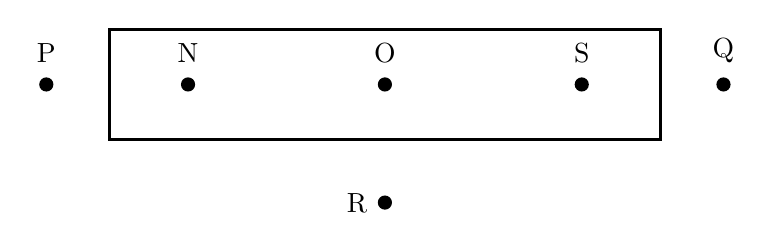
\begin{tikzpicture}
  % bar (rectangle)
  \draw[line width=1.2pt] (0,0) rectangle (7,1.4);
  % interior points N, O, S on centreline
  \foreach \x/\lab in {1/N,3.5/O,6/S}{
    \fill (\x,0.7) circle (0.09);
    \node[above] at (\x,0.85) {\lab};
  }
  % exterior points P (left) and Q (right) on same line
  \fill (-0.8,0.7) circle (0.09);
  \node[above] at (-0.8,0.85) {P};
  \fill (7.8,0.7) circle (0.09);
  \node[above] at (7.8,0.85) {Q};
  % point R below centre
  \fill (3.5,-0.8) circle (0.09);
  \node[left] at (3.4,-0.8) {R};
\end{tikzpicture}
